\documentclass[conference]{IEEEtran}
\IEEEoverridecommandlockouts

\usepackage{cite}
\usepackage{amsmath,amssymb,amsfonts}
\usepackage{graphicx}
\usepackage{textcomp}
\usepackage{xcolor}
\usepackage{booktabs}
\usepackage{multirow}
\usepackage{array}
\usepackage{tikz}
\usetikzlibrary{positioning,arrows.meta,shapes.geometric,fit,backgrounds,calc}
\usepackage{algorithm}
\usepackage{algpseudocode}
\usepackage[hidelinks]{hyperref}

\newcommand{\status}[1]{\textsc{#1}}

\def\BibTeX{{\rm B\kern-.05em{\sc i\kern-.025em b}\kern-.08em
    T\kern-.1667em\lower.7ex\hbox{\sc e}\kern-.125emX}}

\begin{document}

\title{Agentic Pilot: An Evidence-Driven Local Autonomous AI Agent Framework\\for Privacy-Preserving Intelligent Task Automation}

% Author names and affiliations go here before submission (anonymous for double-blind review).
\author{}

\maketitle

\begin{abstract}
LLM-based assistants that operate software on a user's behalf usually send screenshots and page content to hosted models, retain little from one session to the next, and can declare a task finished when it is not. We present Agentic Pilot, an open-source agent that runs its language and vision models locally through Ollama and drives a Chromium browser through Playwright. The agent is a LangGraph state machine in which observation, planning, execution, verification and recovery are separate nodes, and a task may be reported complete only when a completion predicate evaluated on the live page holds; each evaluation is stored with before/after screenshots and a DOM snapshot. Grounding uses a compact DOM manifest first and a local vision model only when the planner cannot act on the DOM. Calls are routed to small models by role, CAPTCHAs halt the task for the user, and high-risk intents require human approval. We formalize the gate and define a false completion rate. On 35 constructed browser end states, the gate withheld completion in 15 of the 22 states that did not satisfy their goal, all of which a dispatch-only rule would accept, and rejected 1 of 13 satisfied states, at a median cost of 33.8\,ms per decision; the seven misses identify specific missing checks. A code-level audit shows which mechanisms are active on the live path. We also design an extension to files, processes and native applications with accessibility-tree grounding, typed postconditions and deterministic permission tiers, and give an end-to-end evaluation protocol for local hardware.
\end{abstract}

\begin{IEEEkeywords}
autonomous agents, large language models, local inference, privacy-preserving computing, task automation, execution verification, human-in-the-loop
\end{IEEEkeywords}

\section{Introduction}
\label{sec:intro}

Assistants built on large language models (LLMs) increasingly act on a user's behalf: they open pages, fill forms and read results. Several of the web and GUI agents reviewed in Section~\ref{sec:related} send each observation, often a full screenshot, to a hosted multimodal model~\cite{he2024webvoyager,zheng2024seeact,zhang2025ufo,zhang2025appagent}. For a personal assistant this is a poor fit. The screen of a logged-in user carries names, messages and account data, and leakage of personal information from language models has been measured even after scrubbing~\cite{lukas2023pii}. Few of these systems keep memory across sessions, and most operate either in a browser or in one other environment rather than across the applications a person uses (Table~\ref{tab:related}).

A second problem is independent of where the model runs. An agent can believe it has finished when it has not. We call this \emph{premature completion}: the agent emits a terminal ``done'' while the environment does not satisfy the user's goal. A typical case is a search request in which the agent opens the search engine, sees the page load without error, and stops before any query is issued. Every individual browser call succeeded; the task did not. Benchmarks that check final environment state show how wide this gap is~\cite{zhou2024webarena,xie2024osworld}, and self-assessment by the model is not a reliable remedy, since intrinsic self-correction without external feedback does not improve, and can degrade, reasoning accuracy~\cite{huang2024cannot}.

This paper describes Agentic Pilot, an open-source agent that runs its language and vision models locally through Ollama and drives a Chromium browser through Playwright. Its central design rule is that a task may be reported complete only when a check on the observed environment state passes, and that the inputs to this check are written to disk as evidence. The agent is structured as an explicit state machine in LangGraph, so that observation, planning, execution, verification and recovery are separate nodes whose transitions can be inspected and logged.

We make the following contributions:
\begin{enumerate}
\item An evidence-gated execution model that separates action dispatch from task completion, formalized as a completion predicate over observations, together with a \emph{false completion rate} (FCR) metric for measuring premature completion (Section~\ref{sec:formal}).
\item The architecture and implementation of a local agent that combines this gate with role-based routing across local models, DOM-first grounding with a vision-model fallback, CAPTCHA detection that halts rather than bypasses, a task-level human approval gate, and persistent per-step evidence (Sections~\ref{sec:arch}--\ref{sec:impl}).
\item A controlled, reproducible study of the completion gate on 35 constructed browser end states, which quantifies both the premature completions it prevents and the ones it misses (Section~\ref{sec:results}).
\item A design for extending the framework from the browser to the local system (files, processes and native applications) with accessibility-tree-first grounding, typed desktop verification predicates and deterministic permission tiers; we state precisely which parts of it exist in code today (Section~\ref{sec:desktop}).
\item A code-level audit of which mechanisms are active on the live execution path, and an end-to-end evaluation protocol with ablations for the author's hardware (Sections~\ref{sec:impl} and~\ref{sec:setup}).
\end{enumerate}

Section~\ref{sec:related} reviews related work. Section~\ref{sec:arch} presents the architecture and Section~\ref{sec:method} the methodology, including the formal model and the local-system extension. Section~\ref{sec:impl} covers the implementation and its status, Section~\ref{sec:setup} the experimental setup and Section~\ref{sec:results} the results. Sections~\ref{sec:security} and~\ref{sec:limits} discuss security and limitations, and Section~\ref{sec:conclusion} concludes.

\section{Related Work}
\label{sec:related}

\paragraph{Reasoning-and-acting agents} ReAct interleaves reasoning with tool actions~\cite{yao2023react}, building on chain-of-thought prompting~\cite{wei2022chain}; Toolformer learns when to call an API~\cite{schick2023toolformer}. Reflexion and RCI let the model critique and retry its own attempts~\cite{shinn2023reflexion,kim2023rci}, and Voyager accumulates skills checked by a model~\cite{wang2024voyager}. In all of these a model decides that a task is finished, and intrinsic self-correction without external feedback does not reliably help~\cite{huang2024cannot}.

\paragraph{Web and computer-use agents and benchmarks} Mind2Web pairs a ranker over Document Object Model (DOM) elements with an LLM~\cite{deng2023mind2web}; WebVoyager drives live sites from screenshots~\cite{he2024webvoyager}; SeeAct finds grounding to be the bottleneck~\cite{zheng2024seeact,yang2023som}. WebArena, VisualWebArena and WorkArena evaluate on self-hosted or remote-hosted applications with functional checks~\cite{zhou2024webarena,koh2024visualwebarena,drouin2024workarena}; OSWorld and Windows Agent Arena do so in real operating systems~\cite{xie2024osworld,bonatti2024waa}. UFO, Agent S and AppAgent control desktop and mobile applications~\cite{zhang2025ufo,agashe2025agents,zhang2025appagent}, and CogAgent, SeeClick, UI-TARS and OmniParser ground actions in screenshots~\cite{hong2024cogagent,cheng2024seeclick,qin2025uitars,lu2024omniparser}. These works say little about when the agent itself may conclude that a task is done.

\paragraph{Completion checking} Benchmark checkers run after the episode. WebVoyager evaluates trajectories with a multimodal judge~\cite{he2024webvoyager}, Pan et al.\ use model-based evaluators to judge and refine agents~\cite{pan2024autonomous}, and Sumyk and Kosovan train a completion judge for macOS applications~\cite{sumyk2025done}. We study a rule over observed state \emph{inside} the loop, record its inputs, and measure its errors (G1, G2); a model judge is complementary.

\paragraph{Memory, security and local inference} Retrieval-augmented generation~\cite{lewis2020rag,reimers2019sbert}, Generative Agents and MemGPT~\cite{park2023generative,packer2023memgpt} manage agent memory. Indirect prompt injection hides instructions in content the agent reads~\cite{greshake2023indirect}; defenses are insufficient in systematic evaluations~\cite{liu2024formalizing}, InjecAgent, AgentDojo, ToolEmu and OS-Harm measure unsafe behavior~\cite{zhan2024injecagent,debenedetti2024agentdojo,ruan2024toolemu,kuntz2025osharm}, and CaMeL separates trusted control flow from untrusted data~\cite{debenedetti2025camel}. Open-weight models such as Qwen2.5 and Qwen2-VL run on consumer hardware~\cite{yang2024qwen25,wang2024qwen2vl,lin2024awq}; surveys list trustworthiness among open problems of LLM agents~\cite{wang2024survey,xi2025rise}. Table~\ref{tab:related} compares representative systems.

\begin{table}[t]
\centering
\caption{Comparison with representative systems, from what each paper reports. Kind: A agent, B benchmark, M model. Environment: W live websites, Wr self-hosted or cached web pages, Ws simulated web, tool or text environment, D desktop OS, Mo mobile. Completion: who decides that a task is done---the agent's model (model), a checker of the benchmark after the episode (benchmark), a model judge after the episode (judge), or a rule over observed state inside the loop (in-loop rule); n/a for systems that do not end tasks. Evid.: persists state artifacts of each step. Mem.: memory across steps or episodes. Open: open-weight models used or supported. Y yes, P partial, N no, n.r. not reported. All listed systems released code.}
\label{tab:related}
\setlength{\tabcolsep}{2.2pt}
\footnotesize
\begin{tabular}{@{}llllccc@{}}
\toprule
System & Kind & Env. & Completion & Evid. & Mem. & Open \\
\midrule
ReAct~\cite{yao2023react}               & A & Ws & model & N & N & N \\
Reflexion~\cite{shinn2023reflexion}     & A & Ws & model$^{a}$ & N & Y & n.r. \\
WebArena~\cite{zhou2024webarena}        & B & Wr & benchmark & n.r. & N & n.r. \\
Mind2Web~\cite{deng2023mind2web}        & B & Wr & n/a & P & N & Y \\
WebVoyager~\cite{he2024webvoyager}      & A & W & model; judge$^{b}$ & Y & N & N \\
SeeAct~\cite{zheng2024seeact}           & A & W, Wr & model & n.r. & N & P \\
OSWorld~\cite{xie2024osworld}           & B & D & benchmark & n.r. & N & Y \\
UFO~\cite{zhang2025ufo}                 & A & D & model & n.r. & P & N \\
AppAgent~\cite{zhang2025appagent}       & A & Mo & model & n.r. & Y & N \\
CogAgent~\cite{hong2024cogagent}        & M & Wr, Mo & n/a & N & N & Y \\
MemGPT~\cite{packer2023memgpt}          & A & n/a & n/a & N & Y & n.r. \\
AgentDojo~\cite{debenedetti2024agentdojo} & B & Ws & benchmark & n.r. & N & Y \\
\midrule
Agentic Pilot (ours)                    & A & W$^{c}$ & in-loop rule & Y & P$^{d}$ & Y \\
\bottomrule
\end{tabular}
\vspace{2pt}

\raggedright\scriptsize
$^{a}$An evaluator gives feedback between trials. $^{b}$Used for evaluation. $^{c}$Implemented backend; a desktop backend is designed (Appendix~\ref{app:computer}) and not integrated; our end-to-end harness uses self-hosted sites (Wr), not yet run with a model. $^{d}$Implemented and retrieved; its effect is not measured.
\end{table}


\section{Problem Formulation}
\label{sec:problem}

\paragraph{Dispatch and completion} The agent observes an environment state $s_t$ through an observation $\Omega(s_t)$ (for the browser: URL, title, element list and screenshot). A planner maps a goal $g$, a plan $P=(g_1,\dots,g_n)$ and the observation to an action $a_t$. Executing it returns a \emph{dispatch flag} $\alpha_t\in\{0,1\}$, which says only that the call returned without error. The agent may report the task complete only when a completion predicate holds on the state observed \emph{after} the action:
\begin{equation}
\Phi(g,s_{t+1},P,\sigma) = \textstyle\bigwedge_{c\in C(g,P)} c(s_{t+1}) \;\wedge\; \pi(P) \;\wedge\; \neg\beta(s_{t+1},\sigma),
\label{eq:phi-general}
\end{equation}
where $C(g,P)$ is the set of postconditions that the goal and plan imply, $\pi(P)$ states that no plan step is pending, and $\beta$ is a blocking condition (a bot-check page, an unapproved high-risk action) with $\sigma$ the approval state. Dispatch does not imply completion, $\alpha_t=1\not\Rightarrow\Phi=1$. Every evaluation of $\Phi$ is stored with the observed values it used. The same form applies to desktop, file and process state, whose postconditions are typed and exact (Appendix~\ref{app:computer}); only the browser instance is implemented.

\paragraph{The implemented browser predicate} $C(g,P)$ is derived from the wording of the request. $\Phi$ is the conjunction of: no browser-error URL, error or ``not found'' title, or redirect to a sign-in page the request did not name ($E$); not still on a search engine's home page when a search, an extraction or a multi-step plan was requested ($H$); a results page carrying the query quoted in $g$ ($Q$); the literal text that $g$ asks to be entered present in an input, exactly if $g$ says ``exactly'' ($T$); for extraction requests, an answer or structured extraction that mentions a content word of $g$ ($X$); and, for multi-step plans, no pending step unless a structured extraction exists ($R$). Each conjunct is instantiated only when its trigger words occur, so for a request that triggers none, $\Phi$ reduces to $\neg E$. A pre-check implements $\beta$ for bot-check pages and halts the task as \textsc{Blocked}. A plan step counts as done when an action other than \texttt{complete} dispatches during it. $\Phi$ has no tunable threshold: its operating point is fixed by the rules, so we characterize the trade-off between false completions and false rejections by removing conjuncts (Section~\ref{sec:res-ablation}) rather than by a curve.

\paragraph{Metrics} Let $\mathcal{T}$ be a set of episodes or end states, $\mathcal{T}_c\subseteq\mathcal{T}$ those reported complete, and $\Phi^{\star}$ an oracle written independently of $\Phi$ (Section~\ref{sec:method}). With $N_{\mathrm{FC}}=\lvert\{\tau\in\mathcal{T}_c:\Phi^{\star}(\tau)=0\}\rvert$ and $N_{\mathrm{FR}}=\lvert\{\tau\in\mathcal{T}\setminus\mathcal{T}_c:\Phi^{\star}(\tau)=1\}\rvert$,
\begin{equation}
\mathrm{FCR} = \frac{N_{\mathrm{FC}}}{\lvert\mathcal{T}_c\rvert}, \quad
\mathrm{FRR} = \frac{N_{\mathrm{FR}}}{\lvert\{\tau\in\mathcal{T}:\Phi^{\star}(\tau)=1\}\rvert}.
\label{eq:fcr}
\end{equation}
Because a dispatch-only rule reports every state complete, we also report the share of unsatisfied states that the gate withholds, $1-N_{\mathrm{FC}}/\lvert\{\tau:\Phi^{\star}(\tau)=0\}\rvert$. FCR alone rewards an agent that never finishes, so the rates are always reported together, as counts with Wilson 95\% intervals~\cite{wilson1927probable}.

\section{Architecture}
\label{sec:arch}

\begin{figure}[t]
\centering
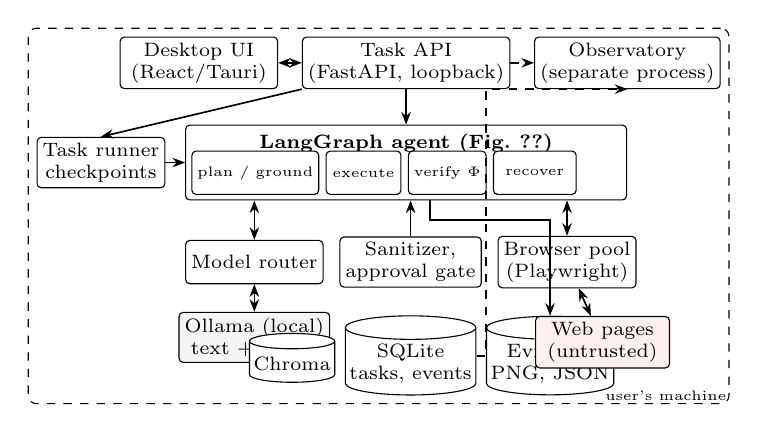
\begin{tikzpicture}[
  font=\scriptsize,
  box/.style={draw, rounded corners=1.5pt, align=center, minimum height=0.55cm, inner sep=2pt, fill=white},
  store/.style={draw, cylinder, shape border rotate=90, aspect=0.18, align=center, minimum height=0.62cm, inner sep=1.5pt, fill=white},
  arr/.style={-{Stealth[length=1.6mm]}, semithick},
  darr/.style={{Stealth[length=1.6mm]}-{Stealth[length=1.6mm]}, semithick},
  node distance=0.28cm and 0.3cm]

% Row 1: user-facing
\node[box, minimum width=2.0cm] (ui) {Desktop UI\\(React/Tauri)};
\node[box, right=of ui, minimum width=2.1cm] (api) {Task API\\(FastAPI, loopback)};
\node[box, right=of api, minimum width=1.7cm] (obs) {Observatory\\(separate process)};

% Row 2: runner + agent
\node[box, below=0.45cm of api, minimum width=5.6cm, minimum height=0.95cm] (agent) {};
\node[anchor=north, font=\scriptsize\bfseries] at (agent.north) {LangGraph agent (Fig.~\ref{fig:graph})};
\node[box, font=\tiny, anchor=south west, minimum width=1.25cm] (plan) at ($(agent.south west)+(0.08,0.07)$) {plan / ground};
\node[box, font=\tiny, right=0.08cm of plan, minimum width=0.95cm] (exec) {execute};
\node[box, font=\tiny, right=0.08cm of exec, minimum width=0.95cm] (ver) {verify $\Phi$};
\node[box, font=\tiny, right=0.08cm of ver, minimum width=1.05cm] (rec) {recover};

\node[box, left=0.25cm of agent, minimum width=1.2cm] (runner) {Task runner\\checkpoints};

% Row 3: services
\node[box, below=0.5cm of agent.south west, anchor=north west, minimum width=1.7cm] (router) {Model router};
\node[box, right=0.2cm of router, minimum width=1.75cm] (sec) {Sanitizer,\\approval gate};
\node[box, right=0.2cm of sec, minimum width=1.7cm] (pool) {Browser pool\\(Playwright)};

% Row 4: local resources
\node[box, below=0.35cm of router, minimum width=1.7cm, fill=gray!8] (ollama) {Ollama (local)\\text + vision};
\node[store, below=0.35cm of sec] (db) {SQLite\\tasks, events};
\node[store, right=0.12cm of db] (ev) {Evidence\\PNG, JSON};
\node[store, left=0.12cm of db] (chroma) {Chroma};
\node[box, below=0.35cm of pool, minimum width=1.7cm, fill=red!6, xshift=0.45cm] (web) {Web pages\\(untrusted)};

% Edges
\draw[darr] (ui) -- (api);
\draw[arr] (api) -- (agent.north -| api);
\draw[arr] (api.south west) ++(0,0) -- (runner.north);
\draw[arr] (runner) -- (agent);
\draw[darr] (router.north) -- (router.north |- agent.south);
\draw[darr] (router) -- (ollama);
\draw[arr] (sec.north) -- (sec.north |- agent.south);
\draw[darr] (pool.north) -- (pool.north |- agent.south);
\draw[darr] (pool) -- (web);
\draw[arr] (agent.south) ++(0.3,0) -- ++(0,-0.25) -| (ev.north);
\draw[arr, dashed] (db.east) ++(0,0.1) -- ++(0.12,0) |- (obs.south);
\draw[arr, dashed] (api.east) -- (obs.west);

% Trust boundary: everything except the web runs on the user's machine
\begin{scope}[on background layer]
\node[draw, dashed, rounded corners=3pt, inner sep=3pt, fit=(ui)(obs)(runner)(ollama)(chroma)(ev)(pool), label={[font=\tiny, anchor=south east, inner sep=1pt]south east:user's machine}] {};
\end{scope}
\end{tikzpicture}
\caption{Components of Agentic Pilot. Everything inside the dashed boundary runs on the user's machine; model inference goes to a local Ollama server. Web pages are the main untrusted input. Dashed arrows are the telemetry feed read by the Observatory.}
\label{fig:arch}
\end{figure}


Fig.~\ref{fig:arch} shows the components. A desktop client submits a natural-language task to a FastAPI service bound to the loopback interface. The task runner executes the control loop, checkpoints its state after every node and cancels tasks that exceed a wall-clock limit (5\,min by default). Task events go to SQLite and to a read-only monitoring process.

\subsection{Control Loop}
\label{sec:loop}

The loop is a compiled LangGraph state machine with eleven nodes; Algorithm~\ref{alg:loop} gives its behavior. A typed state record carries the intent, the plan and step index, the observation, the planned action, the action history, retry and model-call counters, routing decisions and the status. Only the verification step can end a task as \textsc{Completed}, and only when $\Phi$ holds (Fig.~\ref{fig:verify}).

\begin{algorithm}[t]
\caption{Evidence-gated control loop (browser backend)}
\label{alg:loop}
\footnotesize
\begin{algorithmic}[1]
\Require goal $g$; budget of $K{=}15$ model calls
\State $I \gets \Call{ParseIntent}{g}$; $P \gets \Call{Decompose}{g}$ if multi-step
\If{$I$ is high-risk and not approved} \Return \textsc{WaitApproval} \EndIf
\State \Call{Navigate}{$I.\mathit{site}$}; on failure go to line~\ref{alg:recover}
\Loop
  \State $o \gets \Call{Observe}{}$ \Comment{sanitized DOM, screenshot}
  \If{$\beta(o)$} \Return \textsc{Blocked} \Comment{hand off to user} \label{alg:beta}
  \EndIf
  \State $a \gets \Call{Plan}{g, P, o, \textsc{Retrieve}(g)}$ \Comment{model call}
  \State $\alpha \gets \Call{Execute}{a}$; save before/after evidence
  \If{$\alpha = 0$}
    \If{fewer than 3 retries} \textbf{continue} \EndIf
    \State $\textit{st} \gets \Call{Recover}{\text{error}}$ \label{alg:recover}
    \If{$\textit{st}$ is exhausted or blocked} \Return \textsc{Failed} \EndIf
    \State \textbf{continue} \Comment{retry, vision, \dots}
  \EndIf
  \If{$a \neq \texttt{complete}$} mark step done; \textbf{if} steps remain \textbf{continue} \EndIf
  \If{$a = \texttt{complete}$ or last step or text typed}
    \State $(v, \text{obs}) \gets \Phi(g, s, P)$; save as evidence \label{alg:phi}
    \If{$v$} store memory; \Return \textsc{Completed} \EndIf
  \EndIf
  \If{model calls $\geq K$} \Return \textsc{Failed} \EndIf
\EndLoop
\end{algorithmic}
\end{algorithm}


\paragraph{Planning} A small model parses the request into an intent (action, site, target, content, risk level). Requests with a connective or more than eight words are decomposed into steps with an action type and expected outcome. Each iteration, the planner sees the goal, the plan, the current observation and retrieved memory and returns one action. Deterministic rules then adjust it: exact-text requests are grounded to the best visible text field, repeated navigation becomes a failure, and plan steps that name clicking or extracting map to those actions.

\paragraph{Recovery, routing and memory} A failed action is retried through a fresh observation up to three times; later failures are classified into seven types and assigned a strategy (retry, alternative selector, vision fallback, replan), with at most six attempts. Only the vision-fallback strategy changes behavior, by routing the next step to the vision model; the other strategies repeat ordinary planning. A deterministic router assigns each model call a role and the first installed candidate among local Qwen2.5, Qwen3.5 and DeepSeek-R1 models (1.5B--7B parameters), or \texttt{qwen3-vl:2b} and \texttt{moondream} for vision. At termination, outcomes are written to a local Chroma collection and retrieved into later planning prompts.

\begin{figure}[t]
\centering
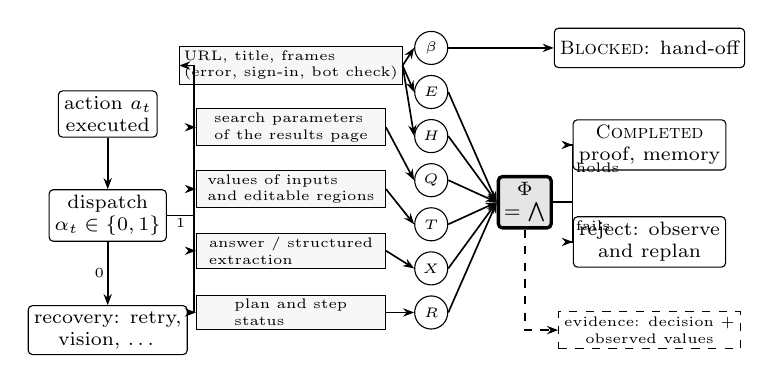
\begin{tikzpicture}[
  x=0.99cm, y=1.12cm,
  font=\scriptsize,
  b/.style={draw, rounded corners=1.5pt, align=center, inner sep=2pt, minimum height=0.5cm, fill=white},
  e/.style={draw, align=left, inner sep=1.5pt, font=\tiny, minimum width=2.4cm, fill=gray!6},
  c/.style={draw, circle, inner sep=0.5pt, minimum size=0.42cm, font=\tiny, fill=white},
  arr/.style={-{Stealth[length=1.4mm]}, semithick},
  lab/.style={font=\tiny, inner sep=1pt}]

\node[b] (act) at (0,0) {action $a_t$\\executed};
\node[b] (alpha) at (0,-1.15) {dispatch\\$\alpha_t\in\{0,1\}$};
\node[b] (rec) at (0,-2.45) {recovery: retry,\\vision, \dots};

\node[e] (ev1) at (2.35, 0.55) {URL, title, frames\\(error, sign-in, bot check)};
\node[e] (ev2) at (2.35,-0.15) {search parameters\\of the results page};
\node[e] (ev3) at (2.35,-0.85) {values of inputs\\and editable regions};
\node[e] (ev4) at (2.35,-1.55) {answer / structured\\extraction};
\node[e] (ev5) at (2.35,-2.25) {plan and step\\status};

\node[c] (cB) at (4.15, 0.75) {$\beta$};
\node[c] (cE) at (4.15, 0.25) {$E$};
\node[c] (cH) at (4.15,-0.25) {$H$};
\node[c] (cQ) at (4.15,-0.75) {$Q$};
\node[c] (cT) at (4.15,-1.25) {$T$};
\node[c] (cX) at (4.15,-1.75) {$X$};
\node[c] (cR) at (4.15,-2.25) {$R$};

\node[b, fill=gray!20, very thick] (and) at (5.35,-1.0) {$\Phi$\\$=\bigwedge$};
\node[b] (ok) at (6.95,-0.35) {\textsc{Completed}\\proof, memory};
\node[b] (no) at (6.95,-1.45) {reject: observe\\and replan};
\node[b] (blk) at (6.95,0.75) {\textsc{Blocked}: hand-off};
\node[draw, dashed, align=center, inner sep=2pt, font=\tiny] (store) at (6.95,-2.45) {evidence: decision +\\observed values};

\draw[arr] (act) -- (alpha);
\draw[arr] (alpha) -- node[lab, left] {0} (rec);
\draw[arr] (alpha.east) -- node[lab, below] {1} ++(0.35,0) |- (ev1.west);
\foreach \n in {ev2,ev3,ev4,ev5} \draw[arr] ($(alpha.east)+(0.35,0)$) |- (\n.west);
\draw[arr] (ev1.east) -- (cB.west); \draw[arr] (ev1.east) -- (cE.west); \draw[arr] (ev1.east) -- (cH.west);
\draw[arr] (ev2.east) -- (cQ.west); \draw[arr] (ev3.east) -- (cT.west);
\draw[arr] (ev4.east) -- (cX.west); \draw[arr] (ev5.east) -- (cR.west);
\foreach \n in {cE,cH,cQ,cT,cX,cR} \draw[arr] (\n.east) -- (and.west);
\draw[arr] (cB.east) -- (blk.west);
\draw[arr] (and.east) -- ++(0.25,0) |- node[lab, right, pos=0.3] {holds} (ok.west);
\draw[arr] (and.east) -- ++(0.25,0) |- node[lab, right, pos=0.3] {fails} (no.west);
\draw[arr, dashed] (and.south) |- (store.west);
\end{tikzpicture}
\caption{Evidence-gated verification after an action (Algorithm~\ref{alg:loop}, lines~\ref{alg:beta} and~\ref{alg:phi}). A failed dispatch goes to recovery and never to $\Phi$. A successful dispatch makes the observed values available to the conjuncts of the browser predicate, each triggered by the wording of the goal (Section~\ref{sec:problem}); the bot-check condition $\beta$ is tested first and hands the task to the user. Every decision is stored with the values it used.}
\label{fig:verify}
\end{figure}


\subsection{Browser Backend}
\label{sec:browser}

A pool of Playwright contexts over one Chromium instance gives each task its own page. Each observation is a DOM pass over interactable elements, recording tag, role, label, up to 120 characters of text, type, visibility, bounding box and selectors; elements are ranked, deduplicated and capped at 50, and their text is passed through a prompt-injection sanitizer. Actions are navigate, click, type, key press, scroll and extract; typed text is read back. The vision model is used only when the planner returns \texttt{need\_help} or recovery requests it: it receives a screenshot and returns a point, which is clicked without an individual check. Per task, the evidence directory holds before/after screenshots of each action, the latest DOM manifest, the verification and recovery records and the node trace.

\section{Implementation}
\label{sec:impl}

The backend is Python (10{,}755 lines, 1{,}682 of them in the graph nodes) on FastAPI, LangGraph, Playwright and Pydantic, with SQLite for tasks and events and a persistent local Chroma store for vectors. The client is React in a Tauri shell; the Observatory is a separate FastAPI service with a React dashboard. The code is public at \url{https://github.com/sudeshsudhii/Agentic-pilot-local}. \todo{AUTHOR: confirm license; archive the evaluated version (tagged release with DOI).}

\paragraph{Design decisions} The runner records each node's name and status in a trace and checkpoints the state after every node, so a task re-scheduled after an approval or a solved CAPTCHA re-enters the graph with its saved plan and skips intent parsing. The completion decision lives in one node; the terminal node adds a guard that downgrades a completion to \textsc{Failed} if the intent named a site but navigation was never verified. Planner output always passes through deterministic rules, which corrects small models on known patterns but places part of the behavior outside the model.

\paragraph{Evidence} Per task, the evidence directory holds before/after screenshots of each executed action, screenshots after navigation and on verified completion, the latest DOM manifest, accumulated verification and recovery records (rewritten on each update, and reset if the file fails to parse), a per-action execution record (action, URLs, screenshots, result, model, role, duration) and the node trace. A retry at the same model-call count overwrites the earlier screenshot pair, a rejected $\Phi$ evaluation keeps no page snapshot of its own, and files carry no integrity protection. Typed text is stored in clear in task events and execution records.

\paragraph{Status audit} Agent documentation tends to run ahead of the code, so we traced each mechanism to the path that executes it (Table~\ref{tab:status}). Most are live. Four are implemented but inert in a normal run: recovery strategies other than re-planning, memory retrieval, the routing cool-down and the verification ablation switch. The repository's evaluation command calls scripts that are not in the repository, its ablation runner imports a function that does not exist, and its certification report counts a task as passed when it ends as completed and any screenshot and trace file exist. We use none of these repository-reported figures as results. The extraction handler, finally, was written for one case study: it formats every extraction as facts about a particular university campus and, when the page yields too few matching lines, substitutes fixed text. It can therefore produce a fabricated answer that satisfies $X$. It must be removed before any end-to-end evaluation.

\begin{table}[t]
\centering
\caption{Status of each mechanism at commit \texttt{eb3803e}, traced through the code. I+T: implemented and unit-tested; I: implemented, untested; P: proposed or partial. Live: affects the default execution path. $^{\dagger}$Changed by the fixes of Section~\ref{sec:impl}.}
\label{tab:status}
\footnotesize
\setlength{\tabcolsep}{2.5pt}
\begin{tabular}{@{}p{3.05cm}ccp{3.3cm}@{}}
\toprule
Mechanism & Status & Live & Note \\
\midrule
Graph, checkpoints, re-scheduling & I+T & yes & graph run only by e2e tests \\
Completion predicate $\Phi^{\dagger}$ & I+T & yes & rule-based (Sec.~\ref{sec:results}) \\
Per-step predicates, click check & P & -- & steps advance on dispatch \\
CAPTCHA halt, resume, fallback$^{\dagger}$ & I+T & yes & no solver \\
DOM grounding, vision fallback & I+T & yes & vision on \texttt{need\_help} \\
Failure classes, retry bounds & I+T & yes & 7 types; 3+3 attempts \\
Recovery strategies$^{\dagger}$ & P & partial & only vision fallback acts \\
Role routing, stickiness$^{\dagger}$ & I+T & yes & task-local; no cool-down \\
Memory and RAG retrieval$^{\dagger}$ & I+T & yes & effect not measured \\
Sanitizer on element text & I+T & yes & title, URL unfiltered \\
Task-level approval gate & I & yes & once per task \\
Model-call audit log & I+T & yes & browsing not logged \\
Evidence store & I+T & yes & some files overwritten \\
Ablation flags, eval runner$^{\dagger}$ & I & yes & not yet run with a model \\
Desktop executor / extension & I / P & no & not wired (Sec.~\ref{sec:desktop}) \\
\bottomrule
\end{tabular}
\end{table}


\section{Evaluation Methodology}
\label{sec:method}

The experiments need no language model. The current-code results were produced on 2026-10-04 on a Linux container with a 4-core Intel Xeon at 2.1\,GHz, 15\,GiB RAM and no GPU, with Python~3.11.15, Playwright~1.56.0, headless Chromium~141 and LangGraph~1.2.12; the decisions of the code before the fixes come from an earlier run on a similar container and are deterministic. Scripts, seeds and raw outputs are under \texttt{artifacts/} and \texttt{benchmarks/e2e/} in the repository.

\subsection{Gate Study}
\label{sec:method-gate}

\paragraph{States and splits} A state is a goal, a URL, an HTML document served through Playwright request interception, the agent's answer and plan state where relevant, and an oracle label. Every state ends with a dispatched action, so a dispatch-only rule accepts all of them. The \emph{design} set (38 states in six categories) was used to find the gate's defects and design the fixes. \emph{Held-out~1} (12 states) was written after the fixes and not used to change them. \emph{Held-out~2} (42 states, 22 unsatisfied) was written to a fixed procedure---varied user phrasings per category, including wordings the gate's trigger lists do not contain, with a balanced split---and committed before the gate was run on it; no gate code changed afterwards. Its SHA-256 is recorded in the repository.

\paragraph{Oracle} The label $\Phi^{\star}$ of a state states whether the goal is achieved by the page and answer shown, judged from the page's facts (for example, whether the answer contains the year in the article). It was written together with the state, before the state was judged by the gate, and it is computed by no code shared with $\Phi$. Its limitation is that one author wrote all states and labels, so no inter-annotator agreement exists; a protocol for independent relabelling with Cohen's $\kappa$~\cite{cohen1960coefficient} is in the repository.

\paragraph{Modes and statistics} Each state is judged by the pre-check and $\Phi$ called directly, and by the real verification node (database, browser-pool and evidence I/O stubbed) with an empty or a generic one-sentence planner reasoning. For the ablation, each conjunct of $\Phi$ and the pre-check $\beta$ is removed in turn by a configuration switch. Counts carry Wilson and Clopper--Pearson 95\% intervals~\cite{wilson1927probable,clopper1934use}; comparisons on the same states use the exact McNemar test~\cite{mcnemar1947note} on discordant pairs. Latency is the median of 20 repetitions after a warm-up.

\subsection{End-to-End Harness}
\label{sec:method-e2e}

\paragraph{Environment and tasks} Live websites change and block automated traffic, and WebArena-style site images were not available offline, so we built five self-hosted sites served on the loopback interface with fictional content that a model cannot answer from memory: a search engine, an encyclopedia, a shop with search and cart, a town-office contact form and newsletter, and a notes application; a further path redirects to a sign-in wall. The 40 tasks (10 development, 30 test) cover search, navigation, text entry, extraction, form submission, multi-step tasks and 5 unsatisfiable requests, at four difficulty tiers by the number of actions a solution needs (1, 2--3, 4--6, more). The notes site appears only in the test split. Tasks needing an account, payment, a CAPTCHA, the live web, or an outcome that neither server state nor answer text can verify were excluded by design.

\paragraph{Oracle} $\Phi^{\star}$ is computed from signals that neither the agent nor $\Phi$ uses: server-side records of the sites (cart contents, form submissions, saved notes, field values autosaved by page scripts), the final URL, and the ground-truth facts in the site data matched against the agent's answer; unsatisfiable tasks are never achieved. It calls no model and shares no code with the verifier. We measured its error rate on 114 scripted trajectories driven directly through Playwright without the agent: a correct solution for each task, an idle trajectory that only opens the start page, and a near miss for 34 tasks (wrong value, wrong item, extra submission, partial query).

\paragraph{Protocol} Table~\ref{tab:e2e} lists the configurations: the full system, two baselines---(a) no completion check and (b) self-verification by the planner model---and one-factor ablations of each conjunct, memory, recovery and each recovery strategy. Each configuration runs in its own process with its own database and memory store, at temperature 0 with a fixed seed, three trials per task, and the same budget of 15 planner calls. Per episode the harness records the oracle verdict, the agent's status, browser actions, model calls and tokens, wall-clock time, each verification decision with its latency, recovery strategies, retrieved memories, Ollama version and model digests, and every host the browser contacted. The analysis reports success, FCR and FRR with Wilson intervals, per-category breakdowns, exact McNemar tests and task-level bootstrap intervals~\cite{efron1979bootstrap} for differences to the full system, and the overhead of $\Phi$ relative to baseline (a). A published agent framework as a third baseline would need its own model and prompts and is left to the authors' runs.

\begin{table}[t]
\centering
\caption{End-to-end evaluation design (implemented in \texttt{benchmarks/e2e}, not yet run with a model). Each configuration changes one factor of the full system; all use the same tasks, model, sampling and budget.}
\label{tab:e2e}
\footnotesize
\setlength{\tabcolsep}{2.2pt}
\begin{tabular}{@{}p{2.95cm}p{2.85cm}p{2.6cm}@{}}
\toprule
Configuration & Change & Question \\
\midrule
\texttt{full} & -- & task success, FCR, FRR, cost \\
\texttt{no\_verification} & every completion claim accepted & baseline (a); gain and overhead of $\Phi$ \\
\texttt{self\_verification} & planner model judges its own completion & baseline (b) \\
\texttt{gate\_without\_}$c$ & conjunct $c$ removed & per-evidence ablation \\
\texttt{no\_memory} & memory and RAG off & contribution of memory \\
\texttt{no\_recovery} & failures not retried & contribution of recovery \\
\texttt{recovery\_}$s$\texttt{\_only} & strategy $s$ pinned & per-strategy recovery \\
\texttt{single\_model}, \texttt{vision\_only} & routing off; no element list & routing, grounding \\
\bottomrule
\end{tabular}
\end{table}


\section{Results and Discussion}
\label{sec:results}

\subsection{Completion Gate on Constructed End States}

Table~\ref{tab:gate} reports the gate study. Called directly, the pre-check and $\Phi$ withhold completion in 15 of the 23 unsatisfied states that a dispatch-only rule accepts (search home pages, HTTP error titles, three bot checks, empty or wrong text fields, empty, navigational or ungrounded answers, a pending plan step) and reject 3 of the 15 satisfied ones. Inside the live \texttt{verify} node the gate is weaker. The node marks the current step complete as soon as its action dispatches, so a premature \texttt{complete} at the last step passes the plan check (P1), and it uses the planner's \texttt{reasoning} as the answer when none exists, so with verbose reasoning the empty-answer case passes too (X2). The live gate withholds 14 or 13 of the 23. FCR values depend on our case mix; the case-level outcomes carry the information.

\begin{table}[t]
\centering
\caption{Completion gate on constructed end states. $n^{-}$/$n^{+}$: states that do not / do meet the goal under the oracle. W: unsatisfied states withheld (a dispatch-only rule withholds none); FR: satisfied states rejected; FC/R: false completions over states reported complete (FCR). Brackets: Wilson 95\% intervals. $p$: exact McNemar test against the dispatch-only rule on the same states. Upper block: current gate by category; lower block: totals, including the gate before the fixes. Held-out~2 was frozen in a commit before the gate was run on it. Source: \texttt{gate\_stats.csv}.}
\label{tab:gate}
\footnotesize
\setlength{\tabcolsep}{2.1pt}
\begin{tabular}{@{}lcccccc@{}}
\toprule
 & \multicolumn{3}{c}{Design (38 states)} & \multicolumn{3}{c}{Held-out 2 (42 states)} \\
\cmidrule(lr){2-4}\cmidrule(l){5-7}
Category & $n^{-}$/$n^{+}$ & W & FR & $n^{-}$/$n^{+}$ & W & FR \\
\midrule
Search & 4/3 & 4 & 0 & 3/3 & 2 & 0 \\
Navigation & 6/2 & 5 & 0 & 4/4 & 1 & 0 \\
Bot check & 4/2 & 3 & 0 & 4/2 & 3 & 1 \\
Text entry & 3/3 & 3 & 0 & 3/3 & 1 & 0 \\
Extraction & 4/3 & 4 & 1 & 5/5 & 0 & 0 \\
Multi-step & 2/2 & 1 & 0 & 3/3 & 2 & 0 \\
\bottomrule
\end{tabular}

\vspace{3pt}
\setlength{\tabcolsep}{1.8pt}
\begin{tabular}{@{}llcccc@{}}
\toprule
Set & Gate & W / $n^{-}$ & FR / $n^{+}$ & FC/R & $p$ \\
\midrule
Design & before & 15/23 [.45,.81] & 3/15 [.07,.45] & 8/20 & $<$.001 \\
Design & after & 20/23 [.68,.95] & 1/15 [.01,.30] & 3/17 & $<$.001 \\
Held-out 1 & before & 1/5 [.04,.62] & 1/7 [.03,.51] & 4/10 & 1.0 \\
Held-out 1 & after & 2/5 [.12,.77] & 1/7 [.03,.51] & 3/9 & .50 \\
Held-out 2 & after & 9/22 [.23,.61] & 1/20 [.01,.24] & 13/32 & .004 \\
Held-out 1+2 & after & 11/27 [.25,.59] & 2/27 [.02,.23] & 16/41 & .001 \\
\bottomrule
\end{tabular}
\end{table}


Each remaining false completion has a specific cause. A results page for another query passes because the search check only asks whether the URL is a results page (S7). A soft ``page not found'' and a login redirect match none of the four error titles (N6, N7). An interstitial with none of the 12 challenge phrases passes (C4). A superset of the requested text passes because matching is by substring (T4). Any answer over 40 characters not starting with one of eight verbs counts as an extraction (X4). A click on the wrong element passes because step status comes from dispatch (P3). A request whose wording triggers no conjunct reduces $\Phi$ to the error check (N8). The false rejections are a correct 13-character answer (X6) and two pages wrongly blocked as bot checks, an article titled ``Robot'' (C5) and a login page with a hidden invisible-reCAPTCHA frame (C6). None of the missing checks needs a model call: query comparison, exact matching, answer-to-goal overlap, step predicates from the planner's expected outcome, visibility-aware challenge detection, and an answer field the planner's reasoning cannot fill. The fixtures can serve as their regression suite.

The gate is cheap next to inference: the 33 decisions that evaluate $\Phi$ had a median of 35.2\,ms (maximum 52.5\,ms; each the median of 20 repetitions), and the five that stop at the pre-check took at most 8.2\,ms, mostly spent reading page text through the browser protocol. The fixture pages are small, so real pages will take longer.

\subsection{Routing Behavior}

We evaluated the router at each call site without inference (\texttt{routing\_resolution.csv}). With the default installation (\texttt{qwen2.5:1.5b}, \texttt{moondream}), intent parsing, decomposition, planning and recovery all resolve to \texttt{qwen2.5:1.5b}, three via the fallback chain, but keywords match as substrings, so ``find a guitar guide'' (``gui'') or ``search Google Images'' is routed to \texttt{moondream}. With all configured models installed, isolated calls get their role's first candidate. In the agent's call order, however, stickiness keeps \texttt{deepseek-r1:1.5b}, chosen for intent parsing and profiled as able to plan, for decomposition and planning; recovery switches to \texttt{qwen2.5:7b} although it makes no model call, and that model is then kept for planning. The router also reuses its last choice across tasks, and the vision fallback bypasses it. In our probes the planner model was never selected for planning.

\subsection{Test Suite}

Without Ollama and with a 240\,s per-test timeout, the repository's suite collects 108 tests in 24 files: 104 pass, 4 fail and one module fails to import; the 20 Observatory tests pass, and backend line coverage is 62.0\,\%. Passing tests use no language model: node tests stub the executor and gateway, and the end-to-end tests run the compiled graph only through failure paths and accept a failed task. Two failures need Ollama and one a directory absent from the repository; the fourth, \texttt{test\_action\_failure\_never\_marks\_completed}, which targets the central property, times out headless. The suite supports claims about component behavior, not task success.

\subsection{End-to-End Evaluation}

End-to-end results need a local Ollama installation and live websites, which the drafting environment lacked. \todo{MEASURE: run the protocol of Section~\ref{sec:setup} and report, per configuration, success rate, FCR and false-rejection rate under the oracle, model calls, wall-clock time, recovery success, vision rate and evidence completeness, with 95\% intervals.} \todo{MEASURE: add a case study with before/after screenshots from \texttt{\textasciitilde/.pilot/logs/evidence/<task\_id>/} of a task in which the gate rejected a premature completion and the agent then finished.}

\section{Discussion}
\label{sec:discussion}

\paragraph{What the evidence supports} A rule over observed state, evaluated inside the agent loop, withholds a significant share of premature completions on constructed browser states at a low false-rejection rate and a cost of tens of milliseconds without model calls. Its defects showed up only when it was tested inside the live node, and its coverage on new phrasings is the binding limit. The evidence does not show that the agent completes tasks.

\paragraph{Rules and model judges} The held-out results argue against extending hand-written web rules indefinitely: each rule is keyed to the wording it was written for. Model-based judges~\cite{pan2024autonomous,sumyk2025done} cover broader goals but add inference cost and are models judging models~\cite{huang2024cannot}. The self-verification baseline in our harness measures exactly this alternative on the same tasks. We expect the two to be complementary---exact postconditions where the environment exposes structured state, a judge as a second opinion where it does not---with both inputs kept as evidence.

\paragraph{Auditing an agent} Before the fixes, several advertised mechanisms (strategy-specific recovery, memory retrieval, a verification switch) had no effect, and extraction substituted fixed text, while the test suite passed. A table that separates implemented, integrated, tested and evaluated components (Table~\ref{tab:status}) found these gaps cheaply, and we recommend it as a standard part of agent papers.

\section{Safety, Privacy and Autonomy}
\label{sec:safety}

\paragraph{Threat model} The user and the host are trusted; content the agent reads is not. We consider (i)~instructions injected through web pages~\cite{greshake2023indirect}; (ii)~high-impact actions without consent, such as posting, sending, purchasing or deleting; (iii)~exposure of credentials and of screenshots that show sensitive data; and (iv)~disclosure of user data to parties other than the site the user asked the agent to use, in particular to a model provider. A compromised host, browser or model is out of scope.

\paragraph{Privacy property} We call the system privacy-preserving in this sense: \emph{model inference is restricted to the user's machine, and task records, memory and evidence are stored only on its disk.} The model client refuses a non-loopback endpoint unless the user sets an explicit override, Chroma telemetry is off, and in 70 agent episodes the agent process opened no non-loopback connection (Section~\ref{sec:res-privacy}). The property does not cover: data the user asks the agent to enter on a website, which reaches that website; model weights and Chroma's default embedding model, which are downloaded once; unencrypted local storage; or traffic of a different configuration. The egress test observed the agent's Python process and the browser's page requests, not background traffic of the Chromium binary.

\paragraph{Autonomy and what the implementation provides} The agent acts only in the browser and exposes no file, process or command action. Before navigation, a task whose parsed action is posting, e-mailing, purchasing, deleting or transferring, or whose risk level is high or critical, waits for the user's approval; intent and risk come from the request alone. Bot checks stop the task for the user. A sanitizer replaces 17 instruction-override, delimiter, exfiltration and role-manipulation patterns in element text. The service listens on loopback, and every model call is logged with destination and payload sizes.

\paragraph{What it does not provide} The sanitizer is a fixed denylist, which systematic evaluations find insufficient~\cite{liu2024formalizing}; titles, extracted text and memory are not filtered. The action label and risk level that trigger approval come from a small model and are decided once per task, so an injected instruction that steers the planner to submit a form mid-task is not gated. The API has no authentication, typed text is stored in clear, and screenshots are not redacted. We make no security claim. The browser hides common automation signals; we consider this acceptable only for a personal assistant acting at human pace on its user's requests, and deployments should disable it where a site's terms prohibit automated access.

\section{Limitations and Threats to Validity}
\label{sec:limits}

\paragraph{Internal validity} We wrote all gate fixtures and their labels, and designed the fixes on the same 38 design states, so the post-fix design results are optimistic; the 12 held-out states are a small, partial correction. The live mode stubs the node's I/O and stands in for the planner with an empty or a generic reasoning string, not with model output.

\paragraph{External validity} All measurements concern the browser backend on small, static fixture pages served offline; real pages are larger and change, and latency will grow. No result involves a language model, a live website, a desktop application, a file or a process. The agent is therefore not shown to complete tasks in any environment.

\paragraph{Construct validity} FCR and FRR depend on the oracle, which for real tasks must be written per task and applied blind to the agent's report. The browser predicate is keyed to request wording, so its coverage depends on how users phrase requests; when no keyword fires it reduces to an error check.

\paragraph{System limitations} Planning with 1.5B--7B models is weak, and deterministic overrides, some site-specific, compensate on common patterns. Vision-grounded clicks are not individually checked. Of the recovery strategies only the vision fallback changes behavior. Memory records are thin, and their effect on planning is unmeasured. Evidence files carry no integrity protection, and a retry can overwrite earlier screenshots. The computer backend is a design with an unintegrated prototype.

\section{Future Work}
\label{sec:future}

The first step is to run the released end-to-end protocol with local models, which answers the open questions on task success, the gate's effect on the full agent, the self-verification baseline, memory and recovery. For the gate, we will derive per-step postconditions from the planner's expected outcomes instead of request wording, add a local vision-language judge as a second opinion, and have the held-out states labelled independently. Beyond the browser, the computer backend of Appendix~\ref{app:computer} would extend the gate to desktop applications, files and processes, behind deterministic pre-action permission checks.

\section{Conclusion}
\label{sec:conclusion}

Agentic Pilot is a local browser agent built on the rule that an executed action is not a completed task: it may report completion only when a predicate over the observed page holds, and it keeps the inputs of that decision as evidence. Inside the live loop the predicate withheld most premature completions on the states it was designed on and 41\% on states frozen before testing, at a median of 27\,ms and no model call; its coverage of new phrasings, not its cost, is the limit. Model traffic is restricted to the user's machine, and the end-to-end harness that will measure task success is released with an oracle validated on scripted trajectories.

\section*{Acknowledgment}
An AI system (Anthropic's Claude) assisted with analyzing the source code, implementing the experiment harness, running the reported component experiments, searching and checking references, and drafting the text of this paper. The authors reviewed, verified and revised all content and take full responsibility for it.

\appendices

\section{Computer Backend (Design, Not Implemented)}
\label{app:computer}

The repository contains a desktop executor that wraps PyAutoGUI and psutil, a text-file helper and a file-existence predicate. None is connected to the control loop: no node, action type or API route calls them, and the file helper does not confine paths. The rest of this appendix is a design.

\paragraph{Observation and grounding} The backend would observe the foreground window through its accessibility tree (Windows UI Automation, macOS Accessibility, AT-SPI) into a manifest shaped like the DOM manifest, falling back to a vision model on a window screenshot. File and process actions are grounded in typed state (paths, hashes, process identity).

\paragraph{Postconditions and permission tiers} Each mutating action carries exact postconditions (Table~\ref{tab:post}) captured with before/after values. Because many local actions cannot be undone, a postcondition checked afterwards is no protection on its own, so an \texttt{action\_gate} node between planning and execution would compute a tier from the concrete action: T0 (read-only) runs freely; T1 (reversible, with a recorded inverse) runs automatically only if the user enabled it; T2 (destructive) and T3 (network-capable programs, credentials) always need approval bound to a hash of the exact action. Paths outside allow-listed roots, inline interpreters and privilege elevation would be refused. A design in which untrusted content cannot change the control flow~\cite{debenedetti2025camel} is a stronger alternative.

\begin{table}[t]
\centering
\caption{Completion postconditions by environment and their status in the code. Impl.: implemented and used by the agent; Unit: implemented and unit-tested, not called by the agent; Prop.: proposed design. $h_0$: hash before the action; $(\mathit{pid},t_c)$: process ID and creation time.}
\label{tab:post}
\footnotesize
\setlength{\tabcolsep}{2.2pt}
\begin{tabular}{@{}p{1.25cm}p{5.05cm}l@{}}
\toprule
Env. & Example postcondition & Status \\
\midrule
Browser & no error or sign-in page; results page for the quoted query; requested text present; answer mentions the goal; no pending step & Impl. \\
Browser & bot-check page detected $\Rightarrow$ \textsc{Blocked} & Impl. \\
File & path exists and size $\geq n$ & Unit \\
File & created / overwritten: $\mathrm{sha256}=\mathrm{sha256}(\text{content})$; moved: source absent and $\mathrm{sha256}(\text{dst})=h_0(\text{src})$; trashed: path absent and trash entry present & Prop. \\
Process & launched: $(\mathit{pid},t_c)$ alive; terminated: $(\mathit{pid},t_c)$ gone within a timeout & Prop. \\
Window & foreground title matches; window with title exists & Prop. \\
Desktop UI & accessibility value of a control equals the input; control state contains \textit{checked} & Prop. \\
Read-only & workspace manifest (paths, sizes, mtimes) unchanged & Prop. \\
\bottomrule
\end{tabular}
\end{table}


\section{End-to-End Task Set}
\label{app:tasks}

The 40 tasks (\texttt{benchmarks/e2e/tasks.json}) are distributed as follows (development/test): extraction 2/8, form submission 2/7, multi-step 1/5, navigation 2/2, search 1/2, text entry 1/2, unsatisfiable 1/4; tiers 1--4 contain 3/6, 4/11, 3/12 and 0/1 tasks. The test split uses all five sites; the notes site appears only there. The harness (\texttt{run\_e2e.py}) takes the split, the number of trials and a list of the configurations of Table~\ref{tab:e2e}; the analysis script (\texttt{analyze\_e2e.py}) writes result tables with Wilson intervals, McNemar tests and bootstrap intervals.


\bibliographystyle{IEEEtran}
\bibliography{references}

\end{document}
